\documentclass[11pt]{standalone}
\usepackage{tikz}
\usetikzlibrary{shapes.geometric}
\usetikzlibrary{plotmarks,shapes.multipart}
\usetikzlibrary{arrows.meta,calc,decorations.pathmorphing}
\begin{document} 
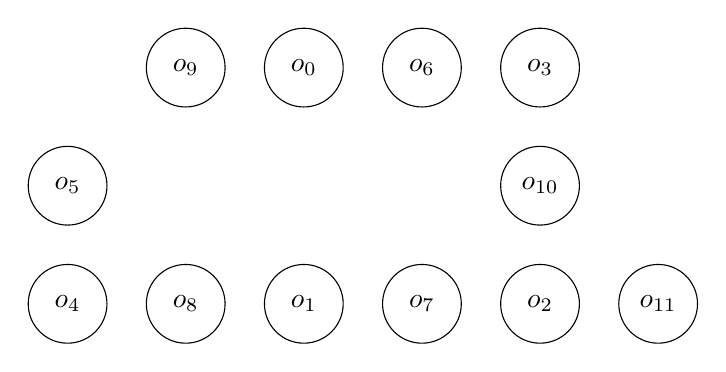
\begin{tikzpicture}
\begin{scope}[local bounding box=scope1,node distance=1.5cm,every node/.style={circle,draw,minimum size=1cm}]

% Nodes
\node[] at(-2.5,0) (o5) {$o_5$};
\node[below of = o5] (o4) {$o_4$};
\node[right of = o4] (o8) {$o_8$};
\node[right of = o8] (o1) {$o_1$};
\node[right of = o1] (o7) {$o_7$};
\node[right of = o7] (o2) {$o_2$};
\node[right of = o2] (o11) {$o_{11}$};
\node[above of = o2] (o10) {$o_{10}$};
\node[above of = o10] (o3) {$o_3$};
\node[left of = o3] (o6) {$o_6$};
\node[left of = o6] (o0) {$o_0$};
\node[left of = o0] (o9) {$o_9$};






\end{scope}



\end{tikzpicture}
\end{document}